\documentclass[10pt,a4paper,openany,twoside,prof]{book}

\usepackage{layout_cours}
\usepackage{hyperref}

\begin{document}
	\chapnumber{4} % numéro du chapitre
	\titre{Nombres réels} % titre du chapitre
	\classe{Seconde} % classe
	\entetegal{}

	% Debut du texte
	% **************
	\vspace{-7mm}
	\paragraph*{Objectif du chapitre:}
	\begin{itemize}
		\vspace{-2mm}
		\setlength\itemsep{-1mm}
		\item
	\end{itemize}
	\vspace{-7mm}

\section{Théorie des ensemble}
\subsection{Union et intersection}
% TODO

\subsection{Intervalles}
% Intervalles de ℝ. Représentation graphique, notations du type [a, +∞[, ] –∞, a], [a, b], etc.
% Représenter un intervalle de la droite numérique. Déterminer si un nombre réel appartient à un intervalle donné.

\begin{defi}{Intervalle borné}{}
	Soit $a, b\in\R$ des réels avec $a\le b$. Soit $I$ l'ensemble des nombres réels compris entre $a$ et $b$. Les extrémités peuvent appartenir à $I$ ou pas. On dit que $I$ est un \bf{intervalle borné}.
\end{defi}

\begin{notation}{}{}
	On note un intervalle avec les extrémités entre crochets. Le crochet est tourné vers l'interieur lorsque l'extrémité appartient à l'intervalle.
\end{notation}

\begin{ex}{}{}
    	$I = \ff{0}{5}$ est l'ensemble des nombres entre 0 et 5. Il y a par exemple $0, \quad 3/5, \quad 4.1235456 \quad$ et $\sqrt{2}$ dedans.


	$J =\fo{0}{\pi}$ est l'ensemble des nombres positifs strictement plus petits que $\pi$.

  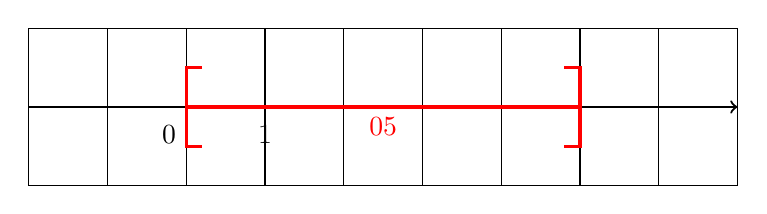
\begin{tikzpicture}
    	\draw (-2,-1) grid (7,1);
    	\draw[->, thick] (-2,0) -- (7,0);
    	\draw[thick] (0, 0.1) -- (0, -0.1) node [below left] {0};
    	\draw[thick] (1, 0.1) -- (1, -0.1) node [below] {1};
    	\draw[red, very thick] (0, 0) --  node [below] {$\ff{0}{5}$} (5, -0);
    	\draw[red, very thick] (0.2, 0.5) --  (0, 0.5) -- (0, -0.5) -- (0.2, -0.5);
    	\draw[red, very thick] (4.8, 0.5) --  (5, 0.5) -- (5, -0.5) -- (4.8, -0.5);
		\end{tikzpicture}

        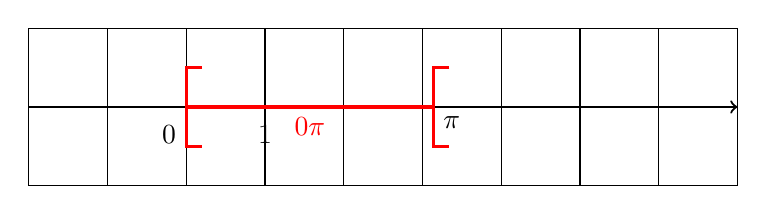
\begin{tikzpicture}
    	\draw (-2,-1) grid (7,1);
    	\draw[->, thick] (-2,0) -- (7,0);
        \node [below right] at (3.14, 0) {$\pi$};
    	\draw[thick] (0, 0.1) -- (0, -0.1) node [below left] {0};
    	\draw[thick] (1, 0.1) -- (1, -0.1) node [below] {1};
    	\draw[red, very thick] (0, 0) --  node [below] {$\fo{0}{\pi}$} (3.14, -0);
    	\draw[red, very thick] (0.2, 0.5) --  (0, 0.5) -- (0, -0.5) -- (0.2, -0.5);
    	\draw[red, very thick] (3.34, 0.5) --  (3.14, 0.5) -- (3.14, -0.5) -- (3.34, -0.5);
		\end{tikzpicture}
\end{ex}

\begin{rem}{}{}
	Un intervalle est donc une partie "sans trous" de l'ensemble des nombres réels $\R$.
\end{rem}

\begin{ex}{}{}
	Il y a donc quatre types d'intervalles bornés:
		\begin{itemize}
			\item L'ensemble des nombres réels $x\in\R$ tels que $a\le x\le b$. On le note $I = \{x\in\R, a\le x\le b\} = \ff{a}{b}$. Les deux extrémités appartiennent à $I$.
			\item  L'ensemble des nombres réels $x\in\R$ tels que $a<x\le b$. On le note $I = \{x\in\R, a< x\le b\}= \of{a}{b}$. $b$ appartient à $I$ mais pas $a$.
			\item L'ensemble $I = \{x\in\R, a\le x< b\}= \fo{a}{b}$.
			\item L'ensemble $I = \{x\in\R, a< x< b\}= \oo{a}{b}$.
		\end{itemize}
\end{ex}



\begin{defi}{Intervalle non borné}{}
	Soit $a\in\R$ un réel. Soit $I$ l'ensemble des nombres réels plus grand que $a$. L'extrémité $a$ peut appartenir à $I$ ou pas. De même, on définit l'ensemble $J$ des nombres réels plus petis que $a$.

	On dit que $I$ et $J$ sont des \bf{intervalles non bornés}.
\end{defi}

\begin{notation}{}{}
	Pour un intervalle non borné, on remplace une extrémité par $+\infty$ ou $-\infty$. Le crochet est toujours ouvert de ce côté, car l'infini n'est pas un nombre réel.
\end{notation}

\begin{exs}{}{}
	$I = \fo{0}{+\infty}$ est l'ensemble des nombres positifs.

	$J = \oo{-\infty}{5}$ est l'ensemble des nombres strictement plus petits que $5$.

    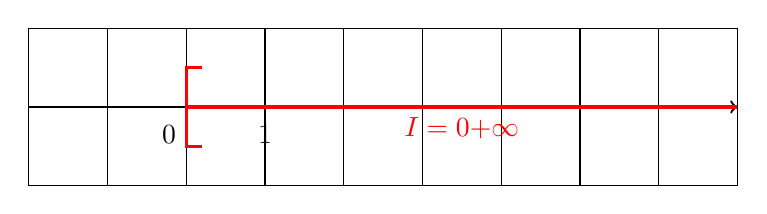
\begin{tikzpicture}
    	\draw (-2,-1) grid (7,1);
    	\draw[->, thick] (-2,0) -- (7,0);
    	\draw[thick] (0, 0.1) -- (0, -0.1) node [below left] {0};
    	\draw[thick] (1, 0.1) -- (1, -0.1) node [below] {1};
    	\draw[red, very thick] (0.2, 0.5) --  (0, 0.5) -- (0, -0.5) -- (0.2, -0.5);
    	\draw[red, very thick] (0, 0) --  node [below] {$I=\fo{0}{+\infty}$} (7, -0);
		\end{tikzpicture}

            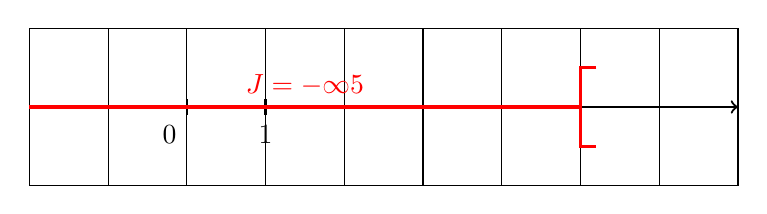
\begin{tikzpicture}
    	\draw (-2,-1) grid (7,1);
    	\draw[->, thick] (-2,0) -- (7,0);
    	\draw[thick] (0, 0.1) -- (0, -0.1) node [below left] {0};
    	\draw[thick] (1, 0.1) -- (1, -0.1) node [below] {1};
    	\draw[red, very thick] (5.2, 0.5) --  (5, 0.5) -- (5, -0.5) -- (5.2, -0.5);
    	\draw[red, very thick] (-2,0) --  node [above] {$J = \oo{-\infty}{5}$} (5, -0);
		\end{tikzpicture}
\end{exs}


\begin{prop}{}{}
	Un intervalle borné correspond à un segment de la droite réelle.

	Un intervalle non borné correspond à une demi-droite ou a la droite réelle entière.
\end{prop}


\section{Puissances d'un nombre}
% Règles de calcul sur les puissances entières relatives, sur les racines carrées.


\section{Valeur absolue}
% Notation en valeur absolue |a| pour la distance de a à 0. Distance entre deux nombres réels.
% Relation √a2 = |a|.

\begin{defi}{Valeur absolue}{}
Soit $a$ un nombre réel.

 On appelle valeur absolue de $a$, notée $|a|$, la distance entre $a$ et $0$. C'est un nombre positif.
\end{defi}

\smallskip
\begin{ex}{}{}
Essayons de déterminer $|-12|$.\medskip

 On sait d'après la définition précédente que $|-12|$ est la \\distance entre $0$ et $-12$. On représente la droite des réels, \\puis (en rouge) la distance entre $0$ et $-12$:

\vspace{-15mm}
\begin{flushright}
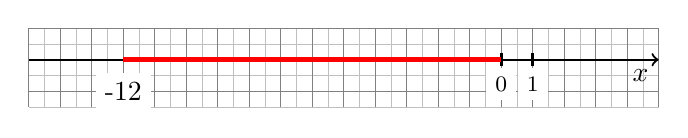
\begin{tikzpicture}[scale=0.4]
\def\xY{-15};
\def\yY{-1.5};
\def\xZ{5};
\def\yZ{1};
\coordinate (Y) at (\xY,\yY);
\coordinate (Z) at (\xZ,\yZ);
\draw[step=0.5cm, lightgray, very thin] (Y) grid (Z);
\draw[step=1cm, gray,thin] (Y) grid (Z);
\draw[ ->,thick] (\xY, 0) -- (\xZ, 0) node[below left]{$x$};
\foreach \x in {0,1}	\draw[very thick](\x,0.2cm)--(\x,-0.2cm) node[below,fill=white]{\footnotesize \x};
\def\xbornea{-12};
\def\orientationa{1};
\draw(\xbornea,-1)node[fill=white]{\xbornea};
\def\xborneb{0};
\def\orientationb{1};
\draw[line width=2pt,red](\xbornea,0)--(\xborneb,0);
\end{tikzpicture}
\end{flushright}

 On trouve |-12|=12.
\end{ex}

\begin{prop}{}{}
  Soit $a\in\R$.
  \begin{itemize}
    \item Si $a\ge0$, alors $|a| =  a$.
    \item si $a\le0$, alors $|a| =  -a$
  \end{itemize}
\end{prop}

\begin{ex}{}{}
  Calculons $\sqrt{a^2}$ pour différentes valeurs de $a$.

  Pour $a=4$, on trouve $\sqrt{4^2} = \sqrt{16} = 4$.

  Pour $a=-3$, on trouve $\sqrt{(-3)^2}=\sqrt{9}=3$.
\end{ex}

\begin{prop}{}{}
    Soit $a\in\R$. Alors $|a|=\sqrt{a^2}$.
\end{prop}

\begin{dem}{}{}
    Soit $a\in\R$. On distingue deux cas.
  \begin{itemize}
    \item Si $a\ge0$, alors d'une part $\sqrt{a^2} = a$ car $a$ est positif. C'est donc bien l'unique nombre positif qui mis au carré donne $a^2$. Dautre part, $|a| =  a$. Donc on a bien $\sqrt{a^2}=|a|$.
    \item Si $a\le0$, on pose $b=-a$. $b$ est donc positif. On calcule alors d'une part, $\sqrt{a^2} = \sqrt{(-a)^2}=\sqrt{b^2} = b$ car $b$ est positif. Dautre part, $|a| =  -a = b$. Donc on a bien $\sqrt{a^2}=|a|$.
  \end{itemize}

\end{dem}

\section{Distance entre les réels}
% Inéquation du type |𝑥 – a| ⩽  r. Représentation graphique des solutions, intervalle [a – r, a + r].

\bigskip
 Plus généralement, avec la notation valeur absolue, il est possible de définir la distance entre deux nombres réels:

\begin{prop}{}{}
Soient $a$ et $b$ deux nombres réels. $|a-b|$ ou $|b-a|$ est la distance entre $a$ et $b$
\end{prop}

\smallskip
\begin{ex}{}{}
Essayons de déterminer $|2-11|$.\medskip

 On sait d'après la définition précédente que $|2-11|$ est la \\distance entre $2$ et $11$. On représente la droite des réel, \\puis (en rouge) la distance entre $2$ et $11$:
\\
\vspace{-19mm}
\begin{flushright}
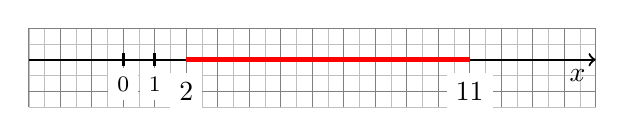
\begin{tikzpicture}[scale=0.4]
\def\xY{-3};
\def\yY{-1.5};
\def\xZ{15};
\def\yZ{1};
\coordinate (Y) at (\xY,\yY);
\coordinate (Z) at (\xZ,\yZ);
\draw[step=0.5cm, lightgray, very thin] (Y) grid (Z);
\draw[step=1cm, gray,thin] (Y) grid (Z);
\draw[ ->,thick] (\xY, 0) -- (\xZ, 0) node[below left]{$x$};
\foreach \x in {0,1}	\draw[very thick](\x,0.2cm)--(\x,-0.2cm) node[below,fill=white]{\footnotesize \x};
\def\xbornea{2};
\def\orientationa{1};
\draw(\xbornea,-1)node[fill=white]{\xbornea};
\def\xborneb{11};
\def\orientationb{1};
\draw(\xborneb,-1)node[fill=white]{\xborneb};
\draw[line width=2pt,red](\xbornea,0)--(\xborneb,0);
\end{tikzpicture}
\end{flushright}

 La distance entre $2$ et $11$ vaut $9$. Donc $|2-11| = 9$
\end{ex}

\end{document}